\documentclass[xcolor={table}]{beamer}
\usepackage{fleqn}
\usepackage{graphicx}
\usepackage{coordsys} %for \numbline commander

%Setup appearance:
\usetheme{Darmstadt}
\usefonttheme[onlylarge]{structurebold}
\setbeamerfont*{frametitle}{size=\normalsize,series=\bfseries}
\setbeamertemplate{navigation symbols}{}
\setbeamertemplate{bibliography item}{[\theenumiv]}

% Standard packages
\usepackage[english]{babel}
\usepackage[latin1]{inputenc}
\usepackage{times}
\usepackage[T1]{fontenc}
\usepackage{multirow}
\usepackage{subfigure}
\usepackage{pbox}
\usepackage{arydshln}
\usepackage{pifont}
\usepackage{cancel}
\usepackage{rotating} % for sideways headings

% Source Code packages
\usepackage{algorithm2e}
\usepackage{algorithmic}

\DeclareSymbolFont{extraup}{U}{zavm}{m}{n}
\DeclareMathSymbol{\varclub}{\mathalpha}{extraup}{84}
\DeclareMathSymbol{\varspade}{\mathalpha}{extraup}{85}
\DeclareMathSymbol{\varheart}{\mathalpha}{extraup}{86}
\DeclareMathSymbol{\vardiamond}{\mathalpha}{extraup}{87}

%%% This section command that adds a big page with section dividers
\usepackage{xifthen}% provides \isempty test
\newcommand{\SectionSlide}[2][]{
	\ifthenelse{\isempty{#1}}
		{\section{#2}\begin{frame} \begin{center}\begin{huge}#2\end{huge}\end{center}\end{frame}}
		{\section[#1]{#2}\begin{frame} \begin{center}\begin{huge}#2\end{huge}\end{center}\end{frame}}
}
%Extends the section slide to to include a shortened section title for the navigation bar as a second parameter
\newcommand{\SectionSlideShortHeader}[3][]{
	\ifthenelse{\isempty{#1}}
		{\section[#3]{#2}\begin{frame} \begin{center}\begin{huge}#2\end{huge}\end{center}\end{frame}}
		{\section[#1]{#2}\begin{frame} \begin{center}\begin{huge}#3\end{huge}\end{center}\end{frame}}
}

\newcommand{\refer}[1]{\footnote{#1}}
\newcommand{\GW}{\text{\textit{Guess-Who~}}}
\newcommand{\keyword}[1]{\alert{\textbf{#1}}\index{#1}}
\newcommand{\firstkeyword}[1]{\textbf{#1}\index{#1}}
\newcommand{\indexkeyword}[1]{\alert{\textbf{#1}\index{#1}}}
\newcommand{\featN}[1]{\textsc{#1}}
\newcommand{\featL}[1]{\textit{'#1'}}
 \newcommand{\ourRef}[1]{\ref{#1} $^{\text{\tiny[\pageref{#1}]}}$}
 \newcommand{\ourEqRef}[1]{\eqref{#1}$^{\text{\tiny[\pageref{#1}]}}$}
  
\DeclareMathOperator*{\argmax}{argmax}
\DeclareMathOperator*{\argmin}{argmin}



\title{The Art of Machine Learning for Predictive Data Analytics}
	\author{John D. Kelleher and Brian Mac Namee and Aoife D'Arcy}
	\institute{}
	\date{}

\begin{document}
\begin{frame}
	\titlepage
\end{frame}
\begin{frame}
	 \tableofcontents
\end{frame}

\begin{frame}
	\begin{itemize}
		\item Predictive data analytics projects use machine learning to build models that capture the relationships in large datasets between descriptive features and a target feature. 
		\item Machine Learning $\approx$ inductive learning
\begin{enumerate}
	\item a model learned by induction is not guaranteed to be correct. 
	\item learning cannot occur unless the learning process is biased in some way. 
\end{enumerate}
	\end{itemize}
\end{frame}

\begin{frame}
	\begin{itemize}
		\item \textit{En masse} all of the questions that must be answered to successfully complete a predictive data analytics project can seem overwhelming.
		\item  This is why we recommend using the  \keyword{CRISP-DM} process to manage a project through its lifecycle.
	\end{itemize}
\end{frame}

 \begin{frame}[plain]
\begin{table}
\renewcommand{\arraystretch}{1.5}
\resizebox{\textwidth}{!}{
\begin{tabular}{p{3.5cm} p{7cm} p{3cm}}
\hline
CRISP-DM & Open Questions & Chapter \\
\hline
\pbox{3.5cm}{Business \\ Understanding} & \textit{What is the organizational problem being addressed? In what ways could a prediction model address the organizational problem? Do we have situational fluency? What is the capacity of the organization to utilize the output of a prediction model? What data is available?} &  Chapter 2 \\
\pbox{3.5cm}{Data \\ Understanding} &  \textit{What is the prediction subject? What are the domain concepts? What is the target feature? What descriptive features will be used?}  &   Chapter 2\\
\hline
\end{tabular}
}
\end{table}
\end{frame} 

 \begin{frame}[plain]
\begin{table}
\renewcommand{\arraystretch}{1.5}
\resizebox{\textwidth}{!}{
\begin{tabular}{p{3.5cm} p{7cm} p{3cm}}
\hline
CRISP-DM & Open Questions & Chapter \\
\hline
\pbox{3.5cm}{Data \\ Preparation} & \begin{minipage}[t]{0.5\columnwidth}
\textit{Are there data quality issues? How will we handle missing values? How will we normalize our features? What features will we include?} \end{minipage}& 
Chapter 3 \\
\pbox{3.5cm}{Modelling \\ ~} & \begin{minipage}[t]{0.5\columnwidth}
\textit{What types of models will we use? How will we set the parameters of the machine learning algorithms? Have underfitting or overfitting occurred?} \end{minipage} & Chapters 4, 5, 6 and 7 \\
\hline
\end{tabular}
}
\end{table}
\end{frame} 

 \begin{frame}[plain]
\begin{table}
\renewcommand{\arraystretch}{1.5}
\resizebox{\textwidth}{!}{
\begin{tabular}{p{3.5cm} p{7cm} p{3cm}}
\hline
CRISP-DM & Open Questions & Chapter \\
\hline
\pbox{3.5cm}{Evaluation \\ ~~} &  \begin{minipage}[t]{0.5\columnwidth}
\textit{What evaluation process will we follow? What performance measures will we use? Is the model fit for purpose?}  \end{minipage} &  Chapter 8\\
\pbox{3.5cm}{Deployment \\ ~~} & \begin{minipage}[t]{0.5\columnwidth} \textit{How will we continue to evaluate the model after deployment? How will the model be integrated into the organization?} \end{minipage} &   Section 8.4.6 and Chapters 9 and 10\\
\hline
\end{tabular}
}
\end{table}
\end{frame} 







\SectionSlide{Different Perspectives on Prediction Models}

\begin{frame} 
\begin{equation}
H(t,\mathcal{D}) = - \sum_{l \in levels(t)} (P(t=l) \times log_2(P(t=l)))
\label{eq:information} 
\end{equation}
\begin{equation}
dist(\mathbf{q},\mathbf{d}) = \sqrt{\sum_{i=1}^{m} (\mathbf{q}[i] -\mathbf{d}[i])^2}
\label{eq:similarity}
\end{equation}
\begin{equation}
P(t=l | \mathbf{q})=\frac{P(\mathbf{q} | t=l)P(t=l)}{P(\mathbf{q})}
\label{eq:probability}
\end{equation}
\begin{equation}
L_2(\mathbb{M}_{\mathbf{w}},\mathcal{D}) =  \frac{1}{2} \sum_{i=1}^{n} (t_i - \mathbb{M}_{\mathbf{w}}(\mathbf{d}_i))^2 
\label{eq:error}
\end{equation}
\end{frame} 

\begin{frame}
	\begin{block}{\keyword{parametric} versus \keyword{non-parametric}}
	\begin{itemize}
		\item  generally describes whether the the size of the \keyword{domain representation} used to define a model is solely determined by the number of features in the domain or if it is affected by the number of instances in the dataset. 
		\item parametric model the size of the domain representation is independent of the number of instances in the dataset (e.g., naive Bayes', regression models)
		\item non-parametric model the number of parameters used by the model increases as the number of instances increases (e.g.,  decision trees)
	\end{itemize}
	\end{block}
\end{frame}


\begin{frame}
	\begin{block}{\keyword{generative} versus \keyword{discriminative}}
	\begin{itemize}
		\item  A model is generative if it can be used to generate data that will have the same characteristics as the dataset from which the model was produced. 
		\item A discriminative models learn the boundary between classes rather than the characteristics of the distributions of the different classes. 
	\end{itemize}
	\end{block}
	\begin{itemize}
		\item Generative and discriminative models attempt to learn different things!
	\end{itemize}
\end{frame}

\begin{frame}
	\begin{block}{A generative model works by:}
	\begin{enumerate}
\item learning $P(\mathbf{d}| t_l)$ (class conditional densities) and  $P(t_l)$; 
\item then using Bayes' theorem to compute $P(t_l| \mathbf{d})$; 
\item applying a decision rule over the class posteriors to return a target level. 
\end{enumerate}
	\end{block}
\end{frame}

\begin{frame}
	\begin{block}{A discriminative model works by:}
\begin{enumerate}
\item learning the class posterior probability $P(t_l|\mathbf{d})$ directly from the data
\item and then applying a decision rule over the class posteriors to return a target level.
\end{enumerate}
	\end{block}
\end{frame}

 \begin{frame} 
\begin{figure}
\centerline{
\begin{tabular}{cc}
\subfigure[]{\label{fig:genVDisc1}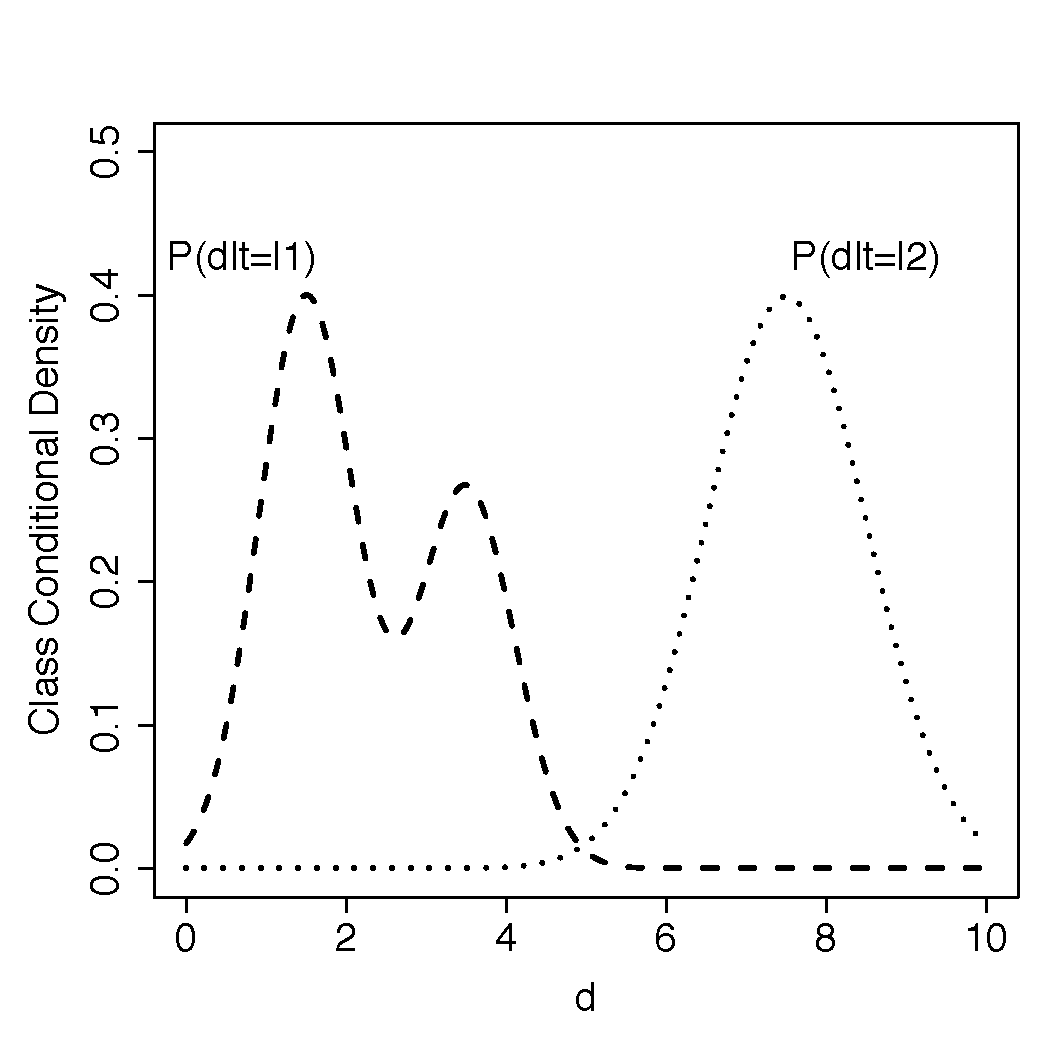
\includegraphics[width=0.45\textwidth]{./images/genVDisc_1.pdf}}&
\subfigure[]{\label{fig:genVDisc2}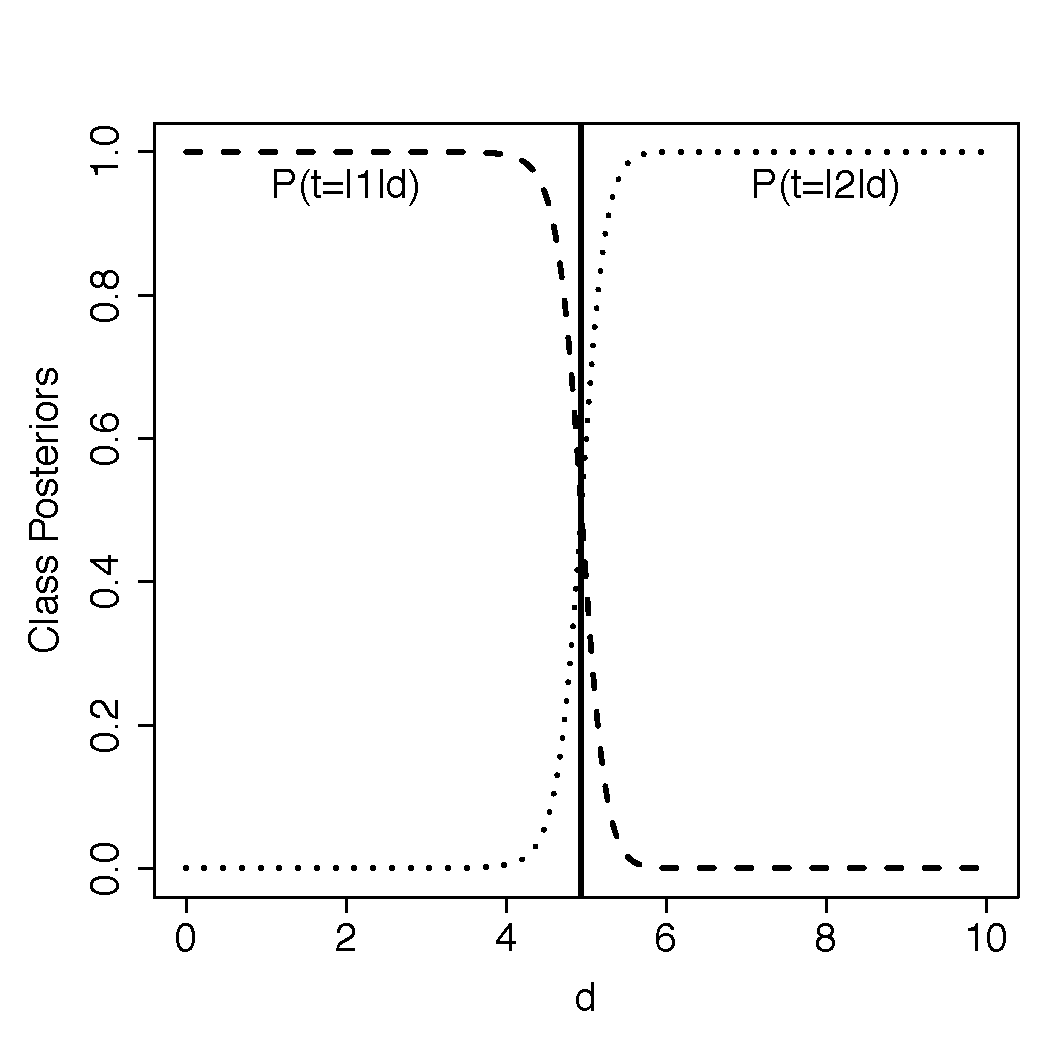
\includegraphics[width=0.45\textwidth]{./images/genVDisc_2.pdf}}\\
\end{tabular}
}
\caption{(a) The class conditional densities for two classes (\featL{l1},\featL{l2}) with a single descriptive feature $\mathbf{d}$. (b) The class posterior probabilities plotted for each class for different values of $\mathbf{d}$. $P(t=\featL{l1}| \mathbf{d})$ is not affected by the multimodal structure of the corresponding class conditional density $P(\mathbf{d}| t=\featL{l1})$.  Based on Figure 1.27 from (Bishop, 2006).}
\label{fig:generativeVdiscriminative}
\end{figure}
\end{frame} 

 \begin{frame} 
\begin{table}
\caption{A taxonomy of models based on the parametric versus non-parametric and generative versus discriminative distinctions.}
\label{tab:modelTaxonomy}
\centering
\begin{footnotesize}
\begin{tabular}{l l l}
\hline
~ & Parametric/ &Generative/\\ 
Model & Non-Parametric &Discriminative\\ 
\hline
k nearest neighbor & Non-Parametric & Generative\\
Decision Trees & Non-Parametric & Discriminative\\
Bagging/Boosting & Parametric\footnote{While the individual models in an ensemble could be non-parametric (for example when decision trees are used) the ensemble model itself is considered parametric.} & Discriminative\\
Naive Bayes & Parametric & Generative\\
Bayesian Network & Parametric & Generative\\
Linear Regression & Parametric & Discriminative\\
Logistic Regression & Parametric & Discriminative\\
SVM & Non-Parametric & Discriminative\\
\hline
\end{tabular}
\end{footnotesize}
\end{table}
\end{frame} 


\SectionSlide{Choosing a Machine Learning Approach}

\begin{frame}
	\begin{itemize}
		\item there is not one best approach that always outperforms the others; \alert{no free lunch theorem}.
		\item We can see the assumptions encoded in each algorithm reflected in the distinctive characteristics of the decision boundaries that they learn for categorical prediction tasks.
	\end{itemize}
\end{frame}


 \begin{frame} 
\begin{figure}[!htb]
       \begin{centering}
   \begin{tabular}{cccc}
       \begin{sideways}Data Sets\end{sideways} &
			\subfigure{\label{}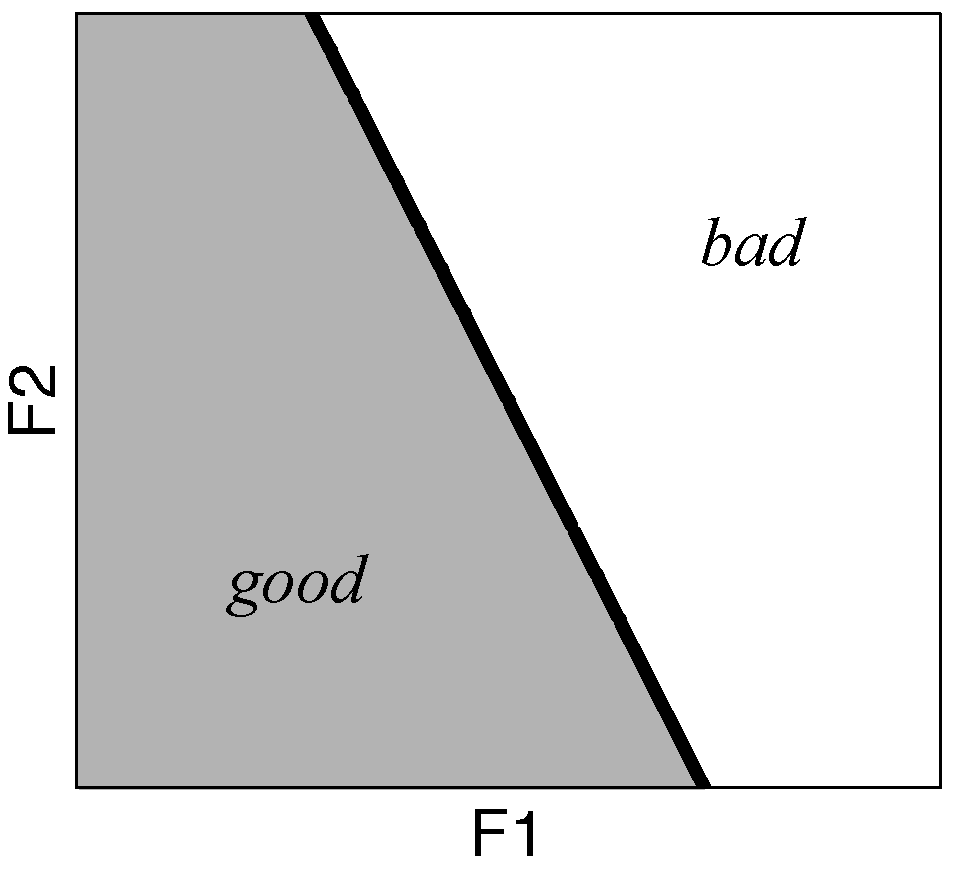
\includegraphics[width=0.29\textwidth]{images/diffContoursDemo_UnderlyingFunction_linear.pdf}} &
			\subfigure{\label{}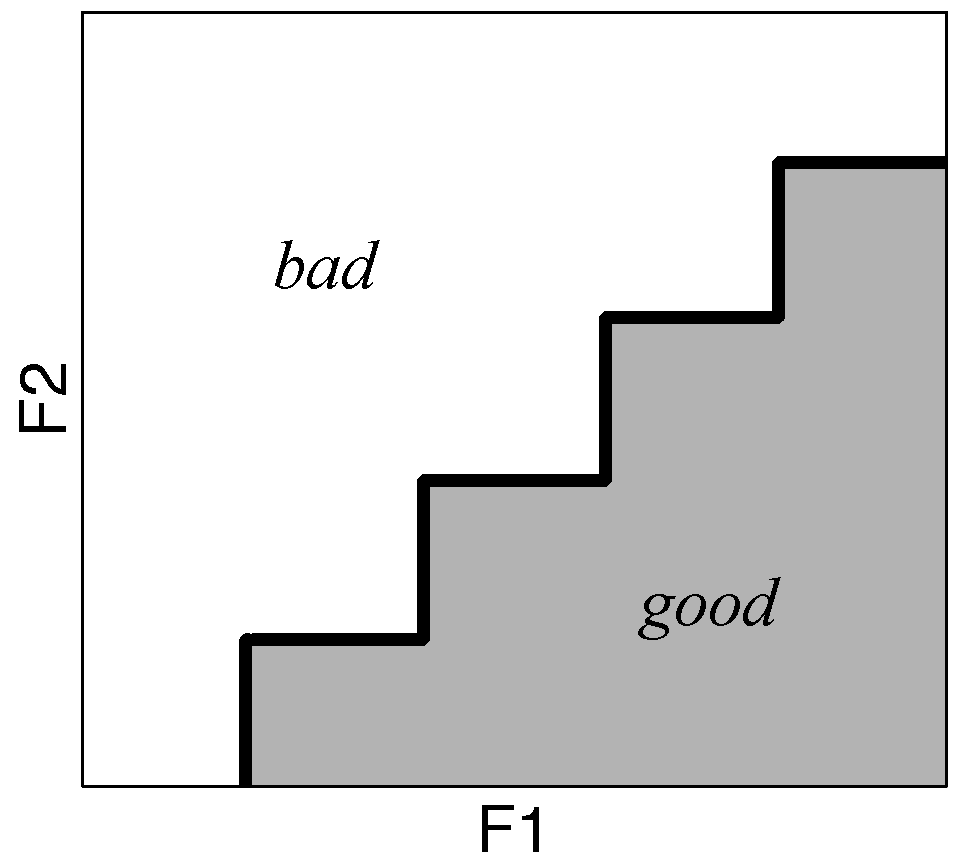
\includegraphics[width=0.29\textwidth]{images/diffContoursDemo_UnderlyingFunction_step.pdf}} &
			\subfigure{\label{}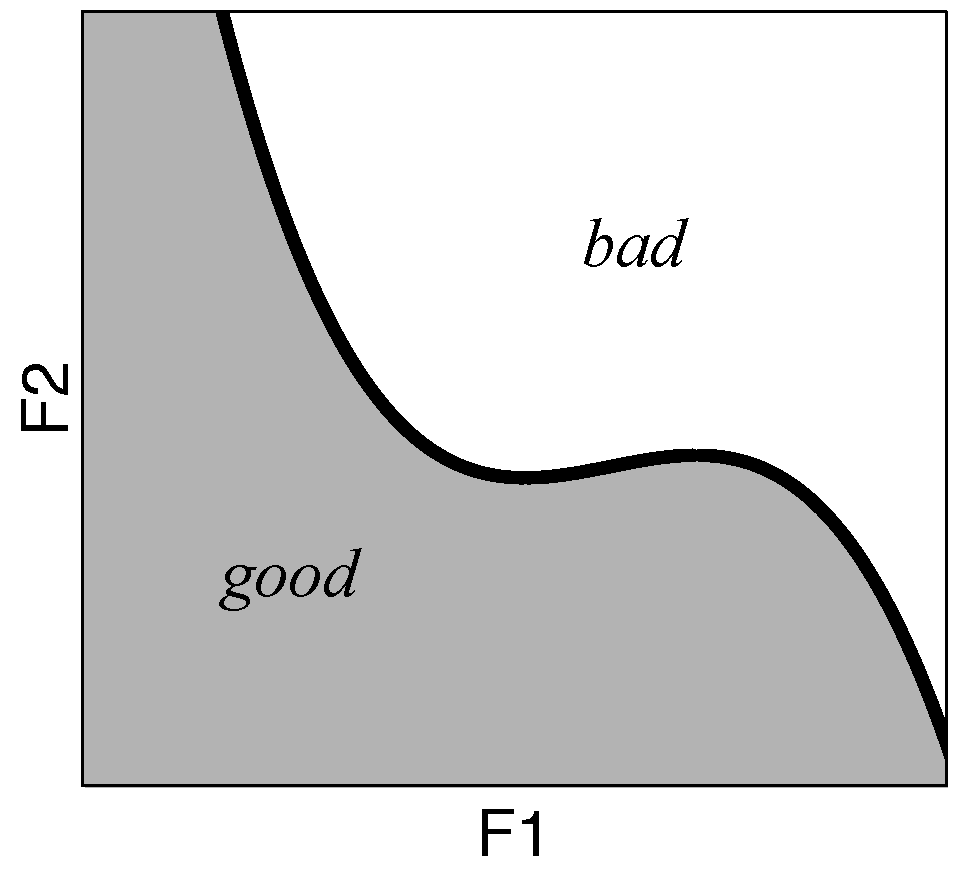
\includegraphics[width=0.29\textwidth]{images/diffContoursDemo_UnderlyingFunction_polynomial3D.pdf}} \\
 \end{tabular}
       \end{centering}
\end{figure}
\end{frame} 



 \begin{frame}[plain]
\begin{figure}[!htb]
       \begin{centering}
   \begin{tabular}{ccc}
			\subfigure{\label{}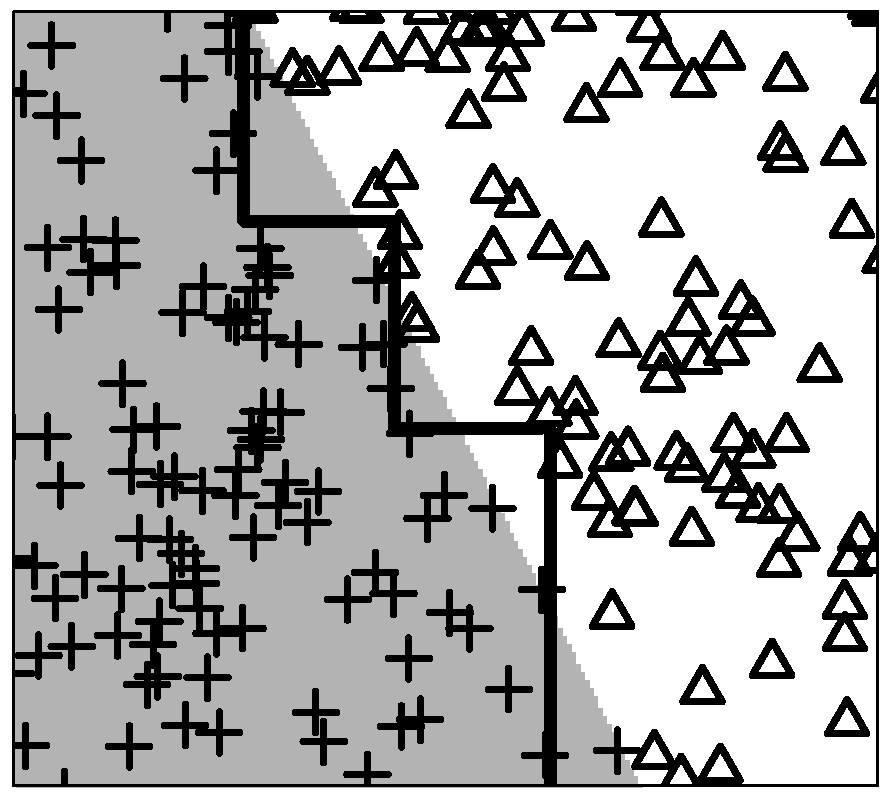
\includegraphics[width=0.2\textwidth]{images/diffContoursDemo_J48_Train_linear}} &
			\subfigure{\label{}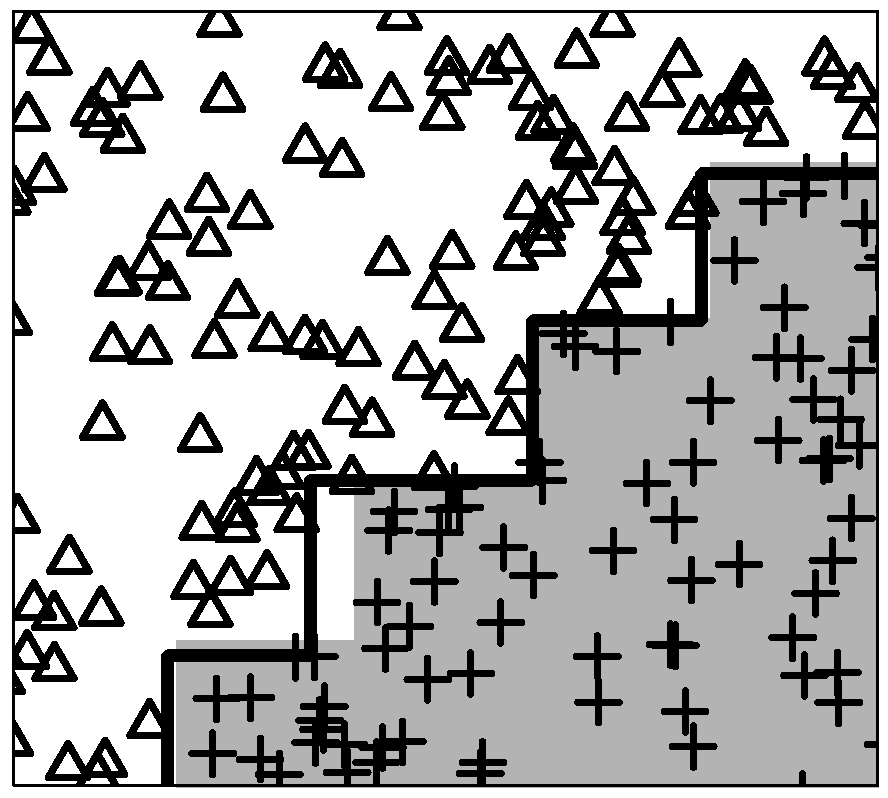
\includegraphics[width=0.2\textwidth]{images/diffContoursDemo_J48_Train_step}} &
			\subfigure{\label{}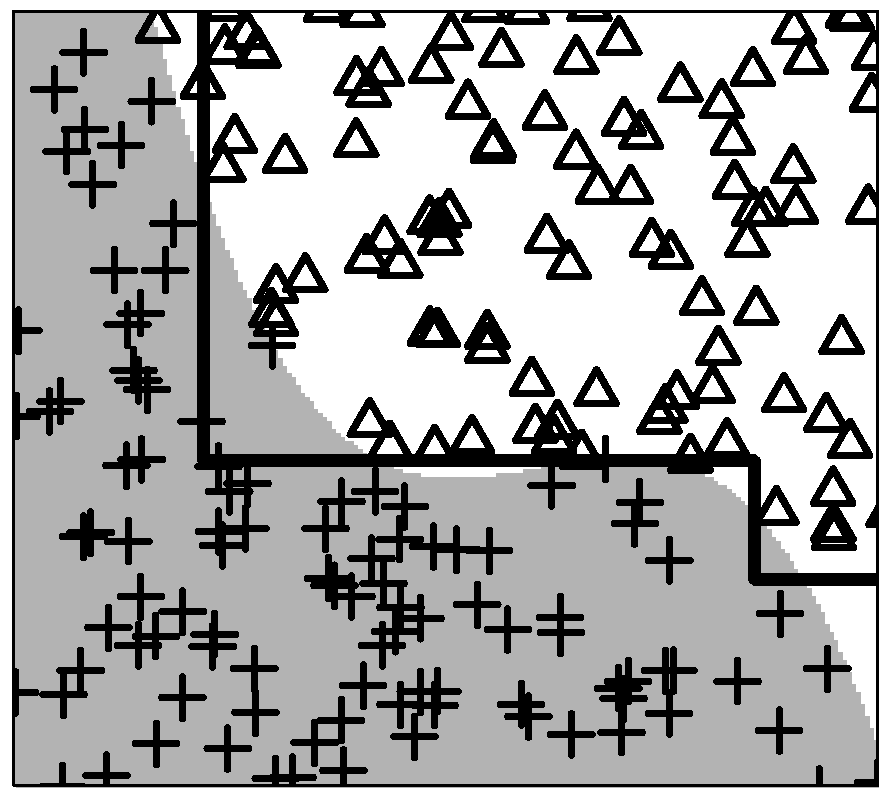
\includegraphics[width=0.2\textwidth]{images/diffContoursDemo_J48_Train_polynomial3D}} \\
			\subfigure{\label{}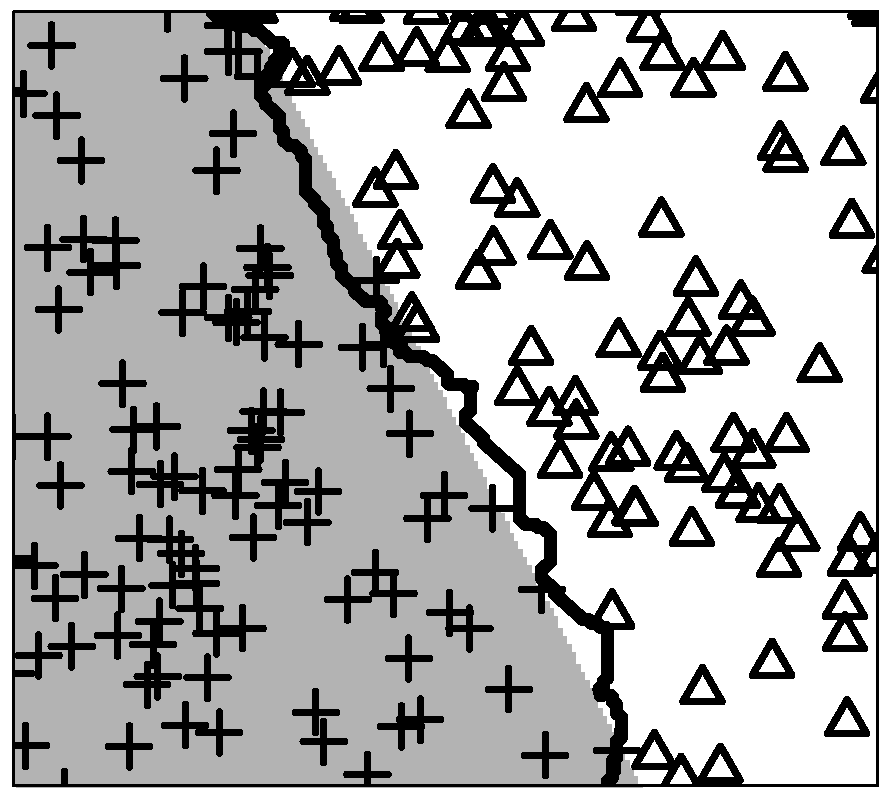
\includegraphics[width=0.2\textwidth]{images/diffContoursDemo_Knn3_Train_linear}} &
			\subfigure{\label{}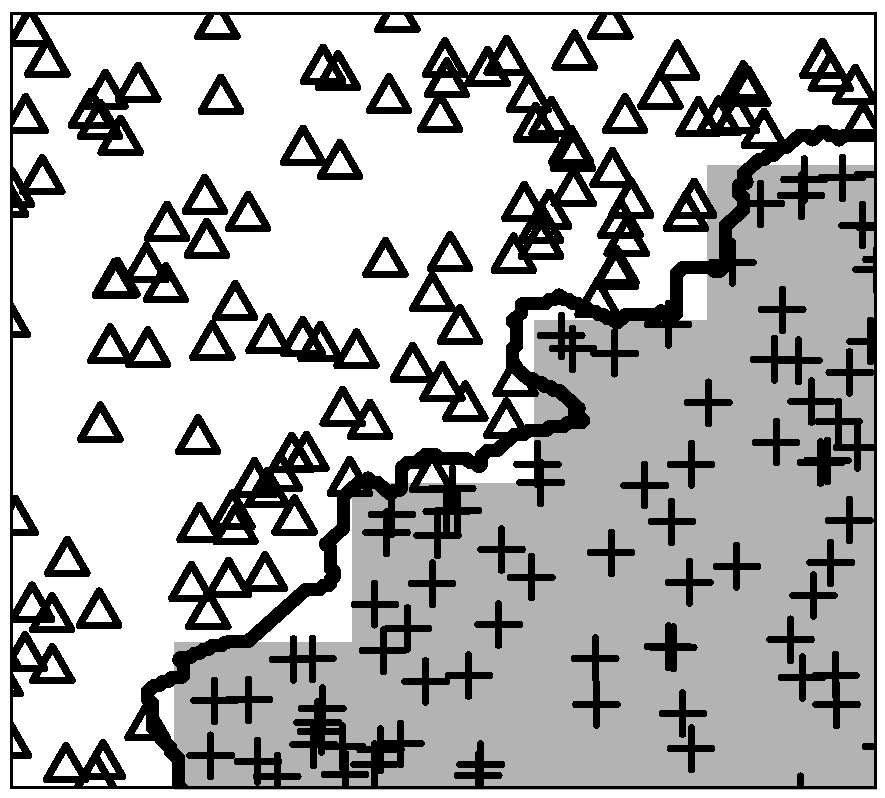
\includegraphics[width=0.2\textwidth]{images/diffContoursDemo_Knn3_Train_step}} &
			\subfigure{\label{}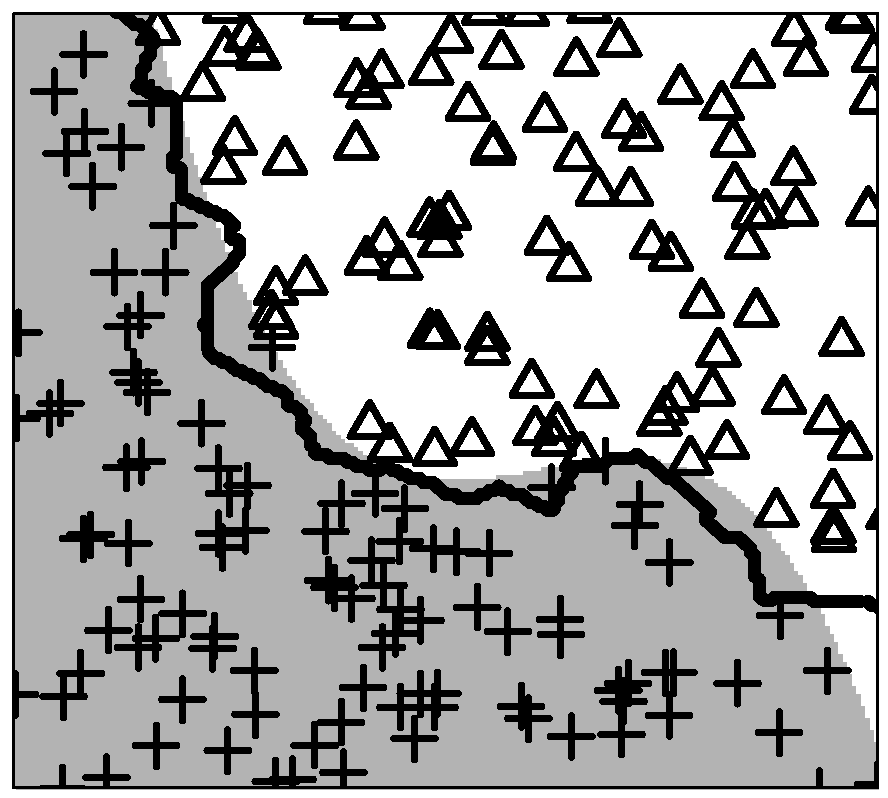
\includegraphics[width=0.2\textwidth]{images/diffContoursDemo_Knn3_Train_polynomial3D}} \\
			\subfigure{\label{}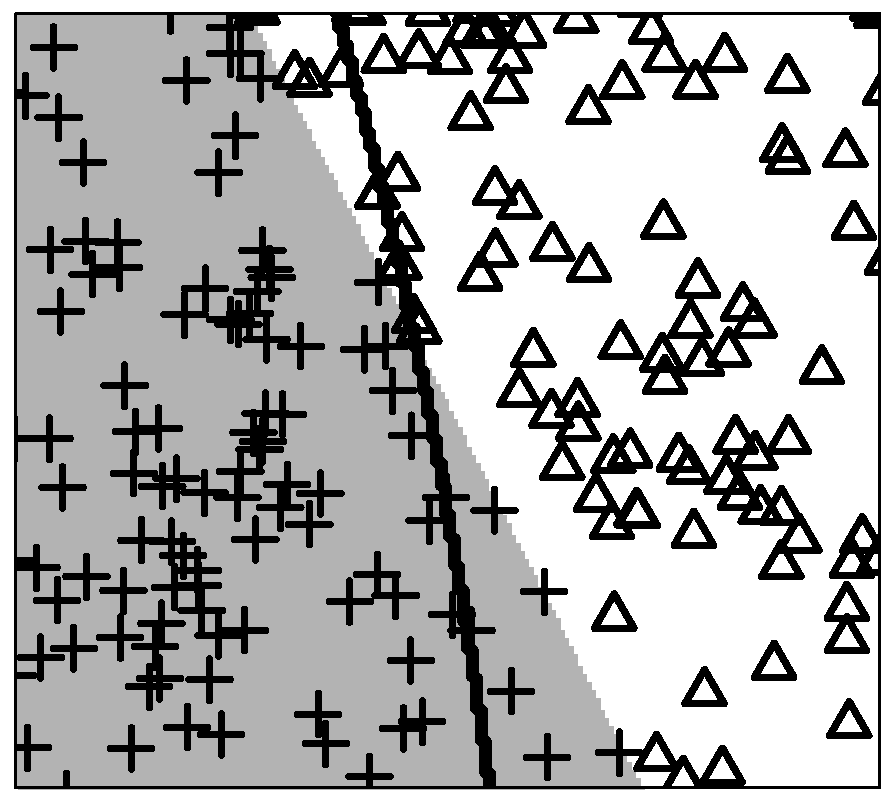
\includegraphics[width=0.2\textwidth]{images/diffContoursDemo_NB_Train_linear}} &
			\subfigure{\label{}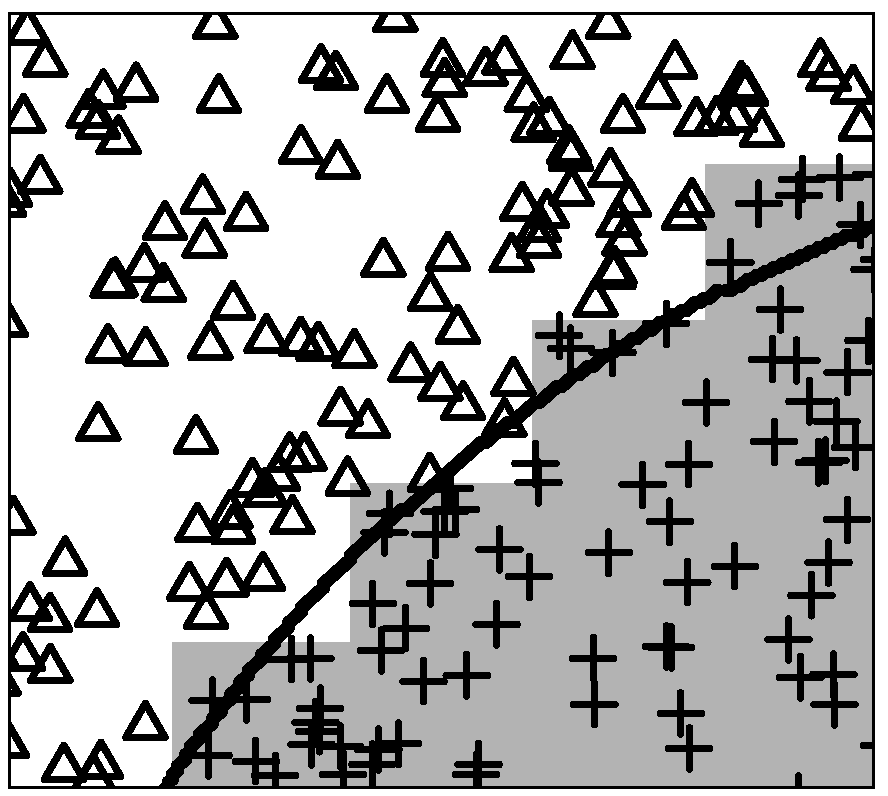
\includegraphics[width=0.2\textwidth]{images/diffContoursDemo_NB_Train_step}} &
			\subfigure{\label{}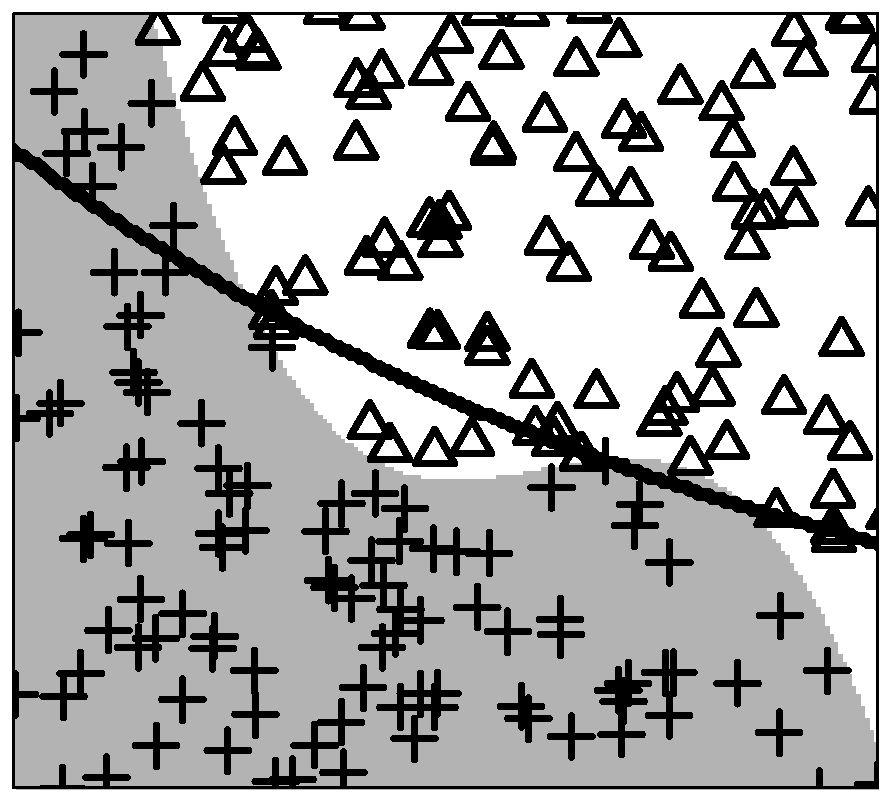
\includegraphics[width=0.2\textwidth]{images/diffContoursDemo_NB_Train_polynomial3D}} \\
			\subfigure{\label{}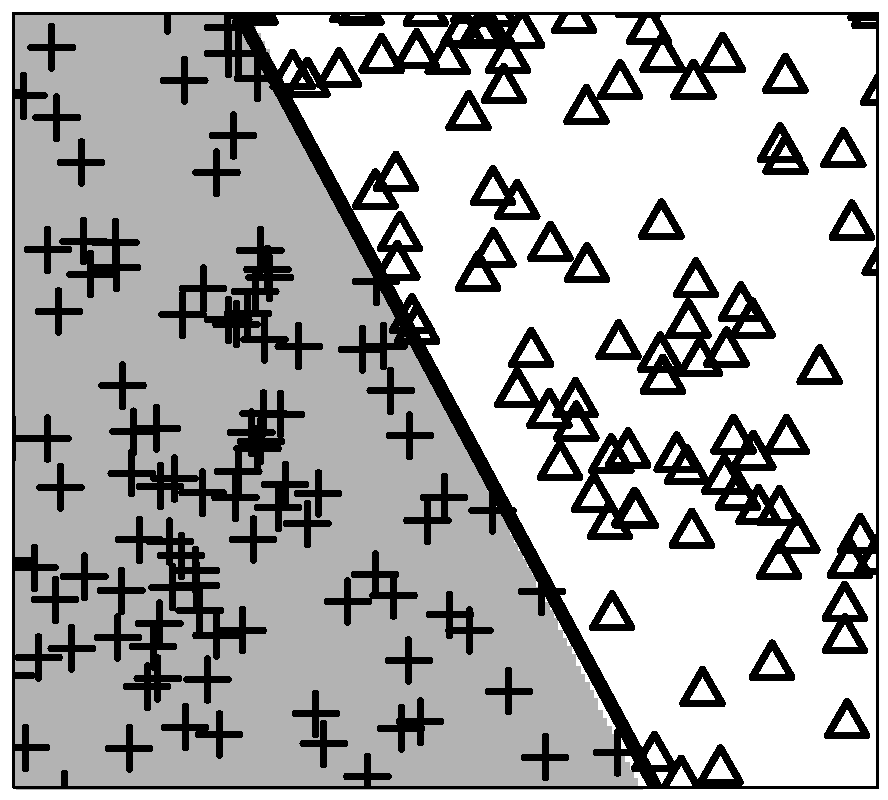
\includegraphics[width=0.2\textwidth]{images/diffContoursDemo_LogReg_Train_linear}} &
			\subfigure{\label{}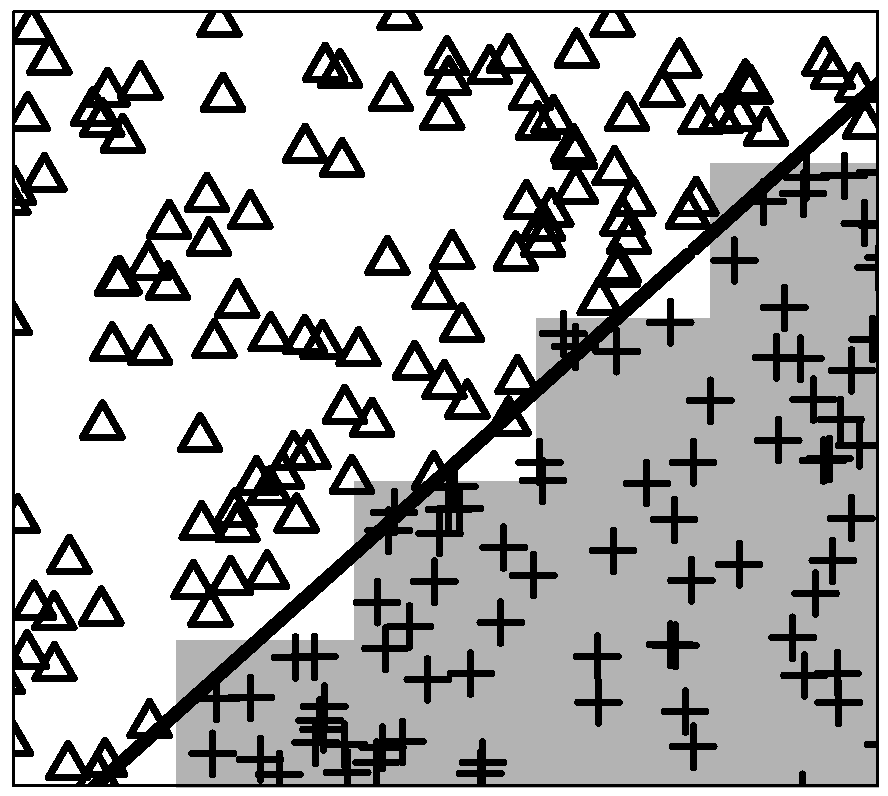
\includegraphics[width=0.2\textwidth]{images/diffContoursDemo_LogReg_Train_step}} &
			\subfigure{\label{}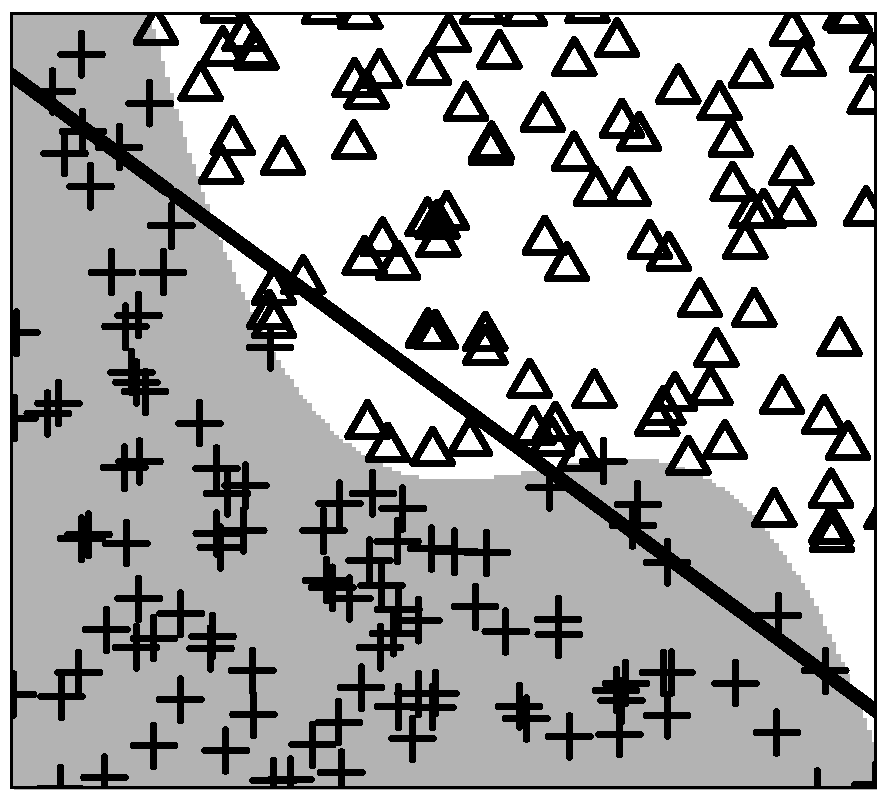
\includegraphics[width=0.2\textwidth]{images/diffContoursDemo_LogReg_Train_polynomial3D}} \\
 \end{tabular}
       \end{centering}
\end{figure}
\end{frame} 

\begin{frame}
	\begin{itemize}
		\item Typically choose a number of different approaches and to run experiments to evaluate which best the particular project. 
		\item There are two questions to consider in the selection of a set of initial approaches:
\begin{enumerate}
	\item Does a machine learning approach match the requirements of the project?
	\item Is the approach suitable for the type of prediction we want to make and the types of descriptive features we are using?
\end{enumerate}
	\end{itemize}
\end{frame}

\subsection{Matching Machine Learning Approaches to Projects}

\begin{frame}
	\begin{block}{Project Requirements}
		\begin{itemize}
			\item Accuracy
			\item Prediction speed
			\item Capacity for retraining
			\item Interpretability
		\end{itemize}
	\end{block}
\end{frame}

\subsection{Matching Machine Learning Approaches to Data}

\begin{frame}
	\begin{block}{Data Considerations}
		\begin{itemize}
			\item continuous target $\rightarrow$ error based models
			\item categorical target $\rightarrow$ information and probability models
			\item continuous descriptive features $\rightarrow$ (+cat. target) similarity based models / (+cont. target) error based models 
			\item categorical descriptive features $\rightarrow$ information and probability models
			\item lots of descriptive features (curse of dimensionality) $\rightarrow$ feature selection
		\end{itemize}
	\end{block}
\end{frame}



\SectionSlide{Your Next Steps}

\begin{frame}
	\begin{itemize}
		\item The easy part of a predictive data analytics project is building the models.
		\item  What makes predictive data analytics difficult, but also fascinating, is figuring out how to answer all the questions that surround the modelling phase of a project.
		\item  Intuition, experience, and experimentation!
	\end{itemize}
\end{frame}


\begin{frame}
\begin{alertblock}{Key tasks for an analyst}
\begin{itemize}
\item become situationally fluent so that we can converse with experts in the application domain; 
\item explore the data to understand it correctly; 
\item spend time cleaning the data; 
\item think hard about the best ways to represent features; 
\item spend time designing the evaluation process correctly.
\end{itemize}
\end{alertblock}
\end{frame}

\begin{frame}
	\begin{itemize}
		\item Machine learning is a huge topic.
		\item There are lots of topics we haven't covered:   \keyword{deep learning}, \keyword{graphical models}, \keyword{multi-label classification},  \keyword{association mining}, \keyword{clustering}, $\mathbf{\dots}$
		\item But, we hope this course has given you the knowledge and skills that you will need to explore machine learning yourself.  
	\end{itemize}
\end{frame}

\begin{frame}
	\tableofcontents
\end{frame}

\end{document}
